%
% ---- contains strange adjustments search "goja"
%

%----------------------------------------------------------------------------------------
%	PACKAGES AND OTHER DOCUMENT CONFIGURATIONS
%----------------------------------------------------------------------------------------

\documentclass[
11pt, % Main document font size
a4paper, % Paper type, use 'letterpaper' for US Letter paper
oneside, % One page layout (no page indentation)
%twoside, % Two page layout (page indentation for binding and different headers)
headinclude,footinclude, % Extra spacing for the header and footer
BCOR5mm, % Binding correction
]{scrartcl}
%%%%%%%%%%%%%%%%%%%%%%%%%%%%%%%%%%%%%%%%%
% Arsclassica Article
% Structure Specification File
%
% This file has been downloaded from:
% http://www.LaTeXTemplates.com
%
% Original author:
% Lorenzo Pantieri (http://www.lorenzopantieri.net) with extensive modifications by:
% Vel (vel@latextemplates.com)
%
% License:
% CC BY-NC-SA 3.0 (http://creativecommons.org/licenses/by-nc-sa/3.0/)
%
%%%%%%%%%%%%%%%%%%%%%%%%%%%%%%%%%%%%%%%%%

%----------------------------------------------------------------------------------------
%	REQUIRED PACKAGES
%----------------------------------------------------------------------------------------

%\usepackage[
%nochapters, % Turn off chapters since this is an article        
%beramono, % Use the Bera Mono font for monospaced text (\texttt)
%eulermath,% Use the Euler font for mathematics
%pdfspacing, % Makes use of pdftex’ letter spacing capabilities via the microtype package
%dottedtoc % Dotted lines leading to the page numbers in the table of contents
%]{classicthesis} % The layout is based on the Classic Thesis style

%\usepackage{arsclassica} % Modifies the Classic Thesis package

\usepackage[T1]{fontenc} % Use 8-bit encoding that has 256 glyphs

\usepackage[utf8]{inputenc} % Required for including letters with accents

\usepackage{graphicx} % Required for including images
\graphicspath{{Figures/}} % Set the default folder for images

\usepackage{enumitem} % Required for manipulating the whitespace between and within lists

\usepackage{lipsum} % Used for inserting dummy 'Lorem ipsum' text into the template

%\usepackage{subfig} % Required for creating figures with multiple parts (subfigures)

\usepackage{amsmath,amssymb,amsthm} % For including math equations, theorems, symbols, etc

\usepackage{varioref} % More descriptive referencing

\usepackage{wrapfig}

\usepackage{caption}

\usepackage{subcaption}

%\usepackage[margin=0.5in]{geometry}

%----------------------------------------------------------------------------------------
%	THEOREM STYLES
%---------------------------------------------------------------------------------------

\theoremstyle{definition} % Define theorem styles here based on the definition style (used for definitions and examples)
\newtheorem{definition}{Definition}

\theoremstyle{plain} % Define theorem styles here based on the plain style (used for theorems, lemmas, propositions)
\newtheorem{theorem}{Theorem}

\theoremstyle{remark} % Define theorem styles here based on the remark style (used for remarks and notes)

%----------------------------------------------------------------------------------------
%	HYPERLINKS
%---------------------------------------------------------------------------------------

%\hypersetup{
%%draft, % Uncomment to remove all links (useful for printing in black and white)
%colorlinks=true, breaklinks=true, bookmarks=true,bookmarksnumbered,
%urlcolor=webbrown, linkcolor=RoyalBlue, citecolor=webgreen, % Link colors
%pdftitle={}, % PDF title
%pdfauthor={\textcopyright}, % PDF Author
%pdfsubject={}, % PDF Subject
%pdfkeywords={}, % PDF Keywords
%pdfcreator={pdfLaTeX}, % PDF Creator
%pdfproducer={LaTeX with hyperref and ClassicThesis} % PDF producer
%}

 % Include the structure.tex file which specified the document structure and layout

%Proposition using definition counter
\newenvironment{proposition}[1][]{\refstepcounter{definition}\par\medskip
   \noindent \textbf{Proposition~\thedefinition. #1} \rmfamily}{\medskip}
 

\begin{document}

%----------------------------------------------------------------------------------------
%	TITLE AND AUTHOR(S)
%----------------------------------------------------------------------------------------

\begin{center}
\begin{huge}
\vspace{1 in}
{\bf  Communication Efficient Data Exchange Among Multiple Nodes}\\  
\end{huge}
\vspace{1 cm}
\begin{large}
\textbf{Midterm Report Summary}\\
\end{large}
\begin{large}
\vspace{0.5cm}
{by\\}
\vspace{0.1cm}
{\textbf{Soumya Subhra Banerjee,} \\ \textit{M.Tech, ECE(CN).} }
\end{large}

\vspace{.2in}

\begin{large}
{ Under the guidance of}\\
\end{large}
\vspace{0.2cm}
\begin{large}
{\textbf{Himanshu Tyagi,}\\ \textit{Assistant Professor, ECE, IISc}}\end{large}
\vspace{1.0cm}

\end{center}





%----------------------------------------------------------------------------------------
%	ABSTRACT
%----------------------------------------------------------------------------------------

\section*{Abstract}
Multiple parties observing correlated data seek to exchange their data using minimum
amount of communication. In case the underlying joint distribution is known, a rate optimal solution to this problem
is offered by Slepian-Wolf compression. In absence of this knowledge, interactive
communication is necessary to attain universal optimality. In both the cases, decoding
is of exponential complexity. However, Slepian-Wolf compression can be implemented
using structured channel codes. In this project, we design rateless Polar codes to enable universal Slepian-Wolf compression and data exchange, when the underlying distribution generating the data is unknown.
 
A key observation driving our project is the similarity between the interactive Slepian-
Wolf compression and the design of an Hybrid ARQ protocol for communication over a
network. Unlike H-ARQ, in our setting, the error-detection capability offered by higher layers
is not available. Hence, we propose a PHY-layer error-detection scheme based
on soft outputs of the Successive Cancellation decoder of Polar codes. We present simulation
results that exhibit the performance of the considered methods. Besides offering a
solution to our problem, this scheme provides a CRC-free Rateless Polar Code which
promises rate gains for short packet length communication and may be of independent
interest.

%----------------------------------------------------------------------------------------
%	PROPOSED SOLUTION
%----------------------------------------------------------------------------------------
\newpage
\section*{Proposed implementation of Recursive Data Exchange} \label{propsol}
Our approach towards implementation of a solution to the \emph{Data-Exchange} problem can be summarised as below, 
\begin{itemize}
\item{Use Rateless Polar Codes with Incremental Freezing to implement RDE.}
\item{Use a PHY layer error detection as retransmission criterion in Incremental Freezing.}
\end{itemize}
\begin{figure}[h]
 \begin{center}
    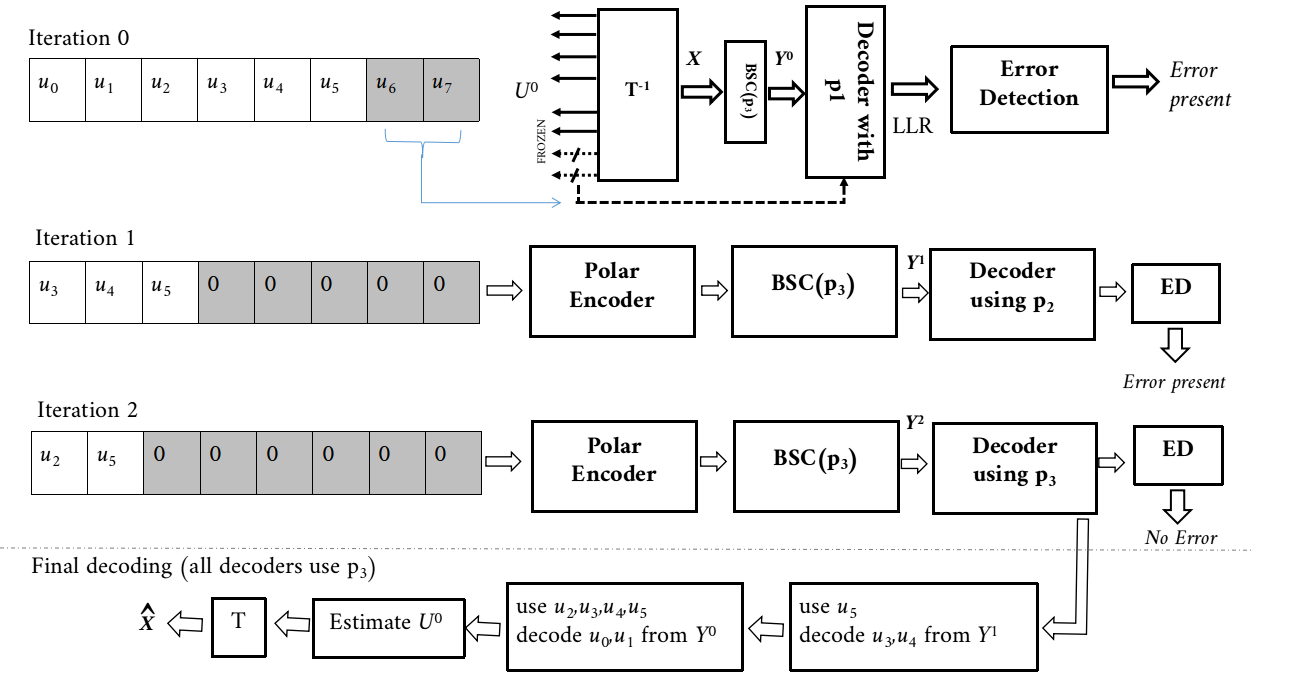
\includegraphics[width=0.7\textwidth]{iswrpc.png}
  \end{center}
  \caption{Iterative SW compression with Incremental Freezing.}
  \label{fig:iswrpc}
\end{figure} 
Here, a compound BSC channel $\mathcal{C}=\{ p_1 \leq p_2 \leq p_3 \leq p_4\}$ is considered, where $p_i$ is the flipover probability of channel $i$. The flipover probability of the true channel is $p_{channel}$.
In the first iteration the scheme guesses the best channel as the true channel and sends the bits that are ought to be frozen with this guess to the receiver over an error-free channel.The decoder uses the log-likelihood ratios for error detection and sends ACK/NACK feedback. In the subsequent iteration the scheme guesses next best channel and the operation is repeated. The scheme terminates on receiving a NACK from receiver or after few iterations. This scheme has been called Incremental Freezing (Inc-Frz).



\subsection*{PHY Layer Error Detection (PHY-ED)} 
Let there be $K$ good bit-channels after polarization $N$ channels.  
Since Inc-Frz guesses the best channel first, we can say that at $j^{th}$ iteration $p_{guess}=p_j$. 
Let $\Lambda_j^i(k)$ be the magnitude of the LLR of $k^{th}$ bit-channel, $k\in{1,2,...N}$ at the output of the decoder at the end of $j^{th}$ iteration such that $p_{guess}=p_j$ for $p_{channel}=p_i$. 
Error detection may be seen as a hypothesis test where,
\begin{align*}
\mathcal{H}_0 & :\text{The channel is the current guess, i.e., } j=i\\
\mathcal{H}_1 & :\text{The channel is worse, i.e., }j<i
\end{align*}
\paragraph{TEST : A given fraction of good channels are above a threshold.}  
In this test $p_{guess}=p_{channel}$ is declared if the |LLR| of a certain fraction of the good channels clear a threshold. The fraction is dependent on the iteration number. After $j^{th}$ iteration,
\begin{align*}  
j &=i,
 \text{   if, } \frac{1}{K}\sum^K_{k=1} \mathbbm{1}_{\{\Lambda_{j}^i(k) > \lambda\}} > \Theta_j \\
j & < i,  \text{ o.w. }
\end{align*} 
The results of Monte-Carlo simulation for estimating $P_M$ and $P_F$ for $\mathcal{C}=\{p_1=0.04,p_2=0.15,p_3=0.2,p_4=0.25\}$ after first iteration is shown in figure \ref{fig:theta1}. Note, in the figures $\Theta$ is considered to be percentage.
\begin{figure}[h!]
 \begin{center}
    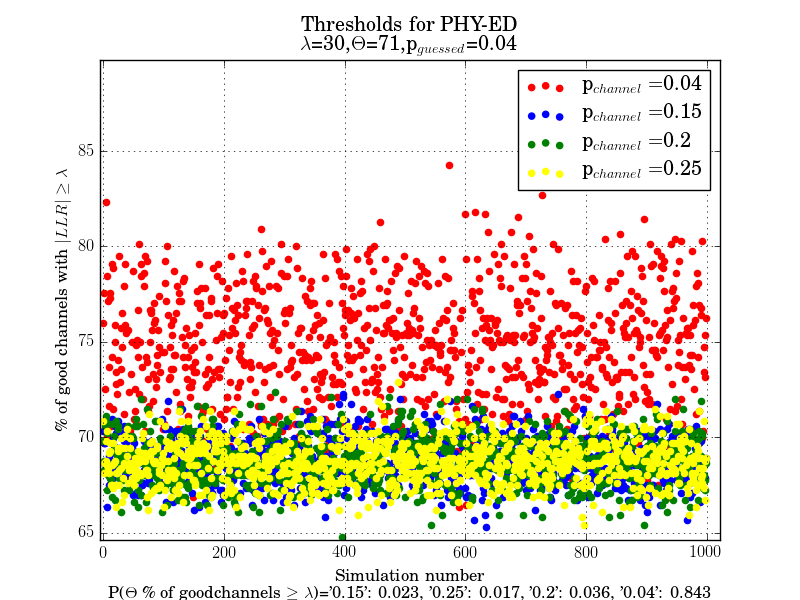
\includegraphics[width=0.7\textwidth]{theta0p04.png}
  \end{center}
  \caption{$P_M$ and $P_F$ estimation for ED after $1^{st}$ iteration, $p_{guess}=0.04$.}
  \label{fig:theta1}
\end{figure}
\subsection*{Performance Evaluation}
%-------------------------------SW
\begin{figure}[h!]
\centering
\begin{subfigure}{.5\textwidth}
 \begin{center}
    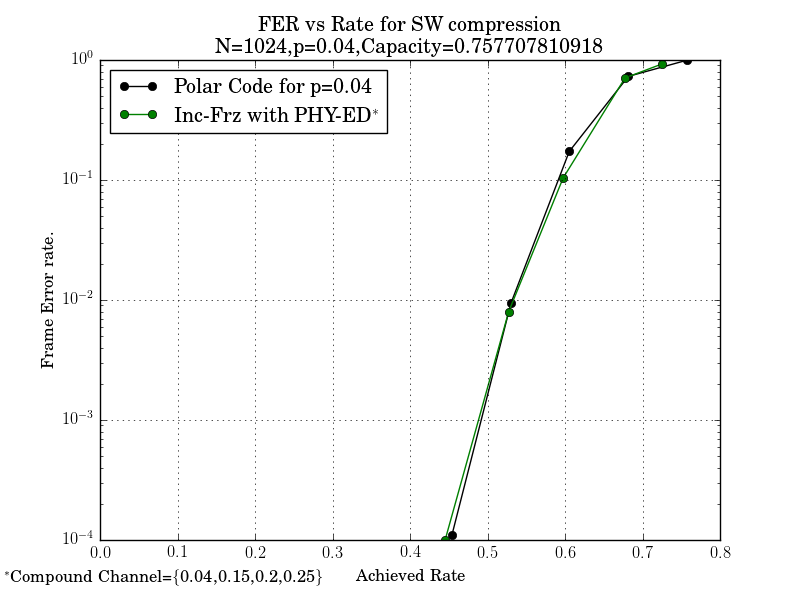
\includegraphics[width=1.1\textwidth]{FERSW_0p04.png}
  \end{center}
  \caption{$p_{channel}=0.04$}
  \label{fig:fersw1}
\end{subfigure}%
\begin{subfigure}{.5\textwidth}
 \begin{center}
    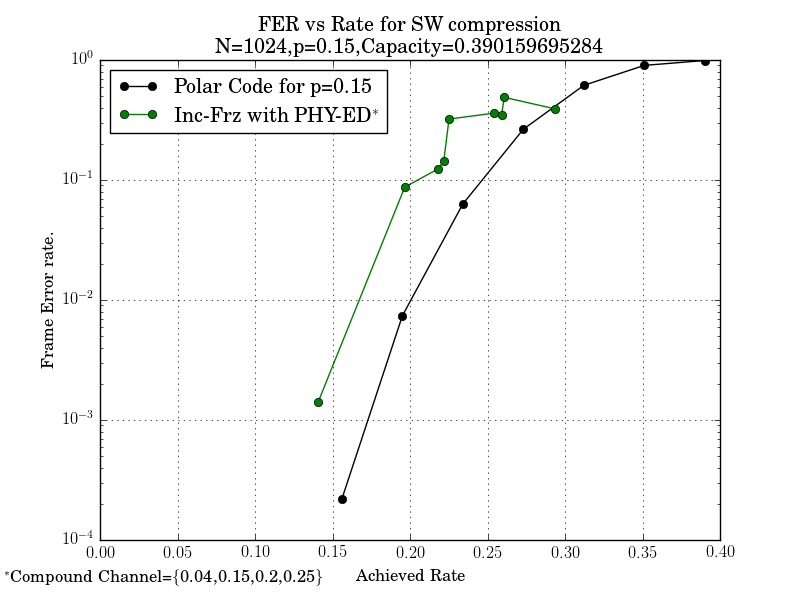
\includegraphics[width=1.1\textwidth]{FERSW_0p15.png}
  \end{center}
  \caption{$p_{channel}=0.15$ }
  \label{fig:fersw2}
\end{subfigure}
\begin{subfigure}{.5\textwidth}
 \begin{center}
    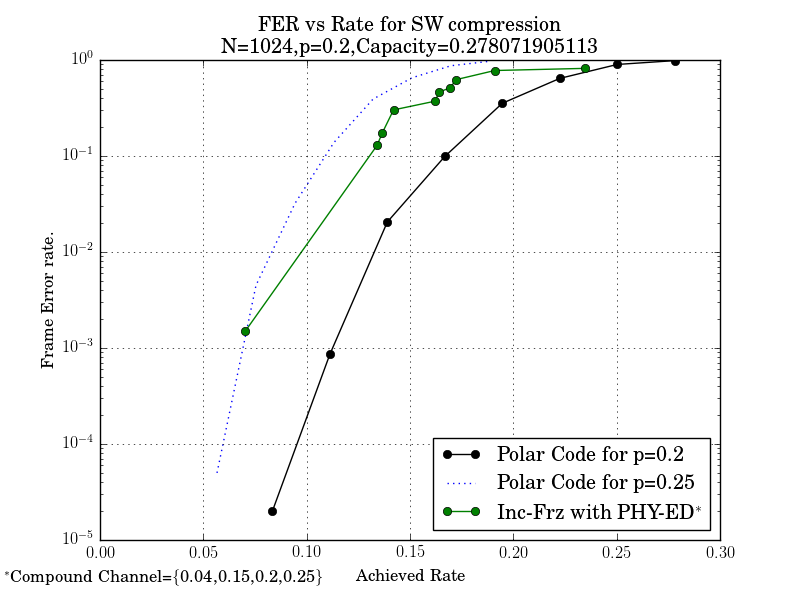
\includegraphics[width=1.1\textwidth]{FERSW_0p2.png}
  \end{center}
  \caption{$p_{channel}=0.2$ }
  \label{fig:fersw3}
\end{subfigure}%
\begin{subfigure}{.5\textwidth}
 \begin{center}
    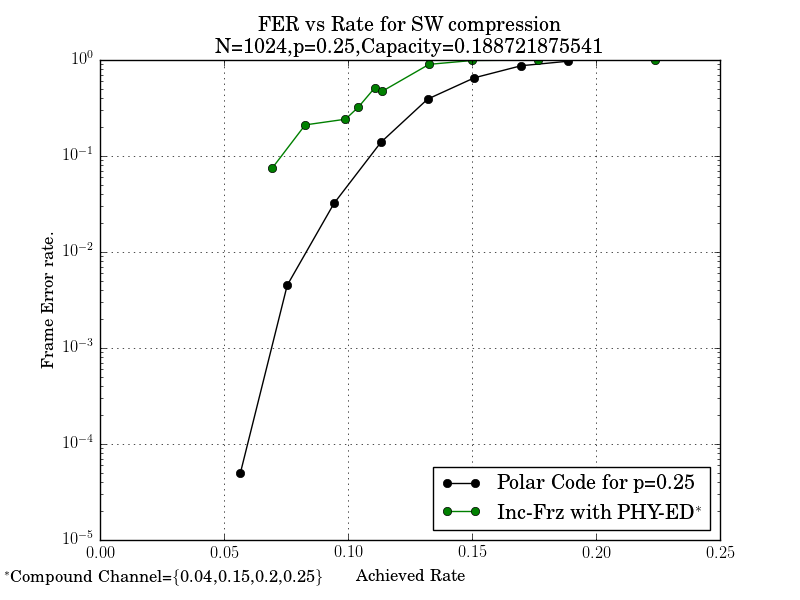
\includegraphics[width=1.1\textwidth]{FERSW_0p25.png}
  \end{center}
  \caption{$p_{channel}=0.25$ }
  \label{fig:fersw4}
\end{subfigure}
\caption{FER vs Rate of SW compression with Inc-Frz and PHY-ED.}
\label{fig:perfsw}
\end{figure}
\begin{figure}[h]
 \begin{center}
    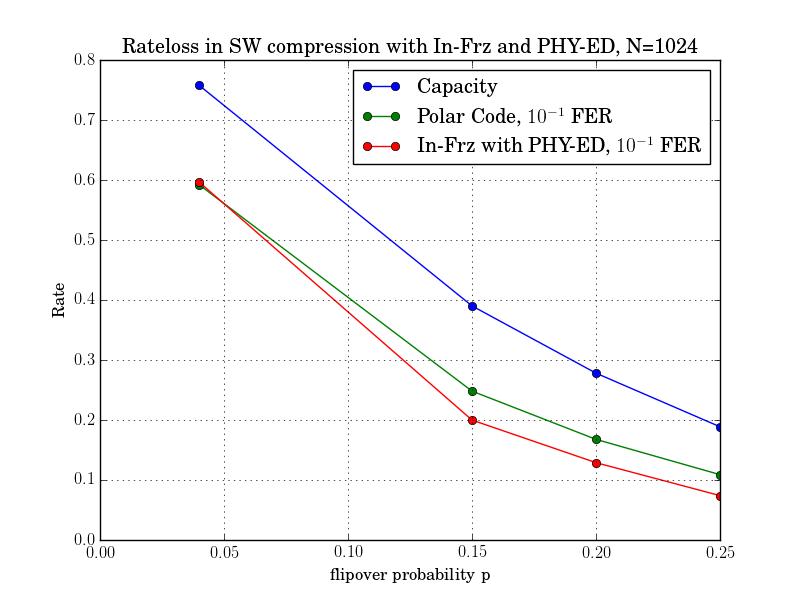
\includegraphics[width=0.7\linewidth]{ratelosssw.png}
  \end{center}
  \caption{Rate loss for SW compression with Inc-Frz.}
  \label{fig:rlsw}
\end{figure}
Simulation results for the scheme in figure \ref{fig:iswrpc} used for iterative SW compression with Inc-Frz and PHY-ED are presented in figure \ref{fig:perfsw}.
Let $K$ be the number of bit-channels assumed to be good at the first iteration. For simulation, $K$ is varied from $0$ to $K^*$ such that $K^*/N$ is the capacity of the best channel. In case of SW compression the number of bits that remain unfrozen after the final iteration divided by $N$ is viewed as the achieved rate. The FER has been plotted against the achieved rates for performance evaluation.

%--------------------------------------------------------------------------
% CONCLUSION AND FUTURE WORK
%--------------------------------------------------------------------------
\section*{Conclusion and Future work}\label{future}
The proposed scheme is an implementable solution to the \emph{Data-Exchange} problem.
It reduces the communication among nodes.
The CRC-free universal polar code promises considerable rate gain for communication using short packet lengths. 
There are few channels which are good for use during the entire transmission. Communicating critical data over these channel ensure high reliability and availability . 
\begin{itemize}
\item Future work.
\begin{itemize}
\item Extensive performance analysis and theoretical analysis of proposed error detection scheme as a RB-HARQ for Polar Codes.
\item Implementation of the scheme for multiparty data exchange.
\end{itemize}
\end{itemize}



%----------------------------------------------------------------------------------------
%	BIBLIOGRAPHY
%----------------------------------------------------------------------------------------
\clearpage
%\renewcommand{\refname}{\spacedlowsmallcaps{References}} % For modifying the bibliography heading

\bibliographystyle{unsrt}

\bibliography{polarmid.bib} % The file containing the bibliography

%----------------------------------------------------------------------------------------

\end{document}